%=============================================================================
%  Kalman Filter for Pairs Trading — Mathematical Notes & Documentation
%  Study Notes + Technical Reference | Dark Wing Project
%=============================================================================
\documentclass[10pt,a4paper,twocolumn]{article}

\usepackage[a4paper,top=1.8cm,bottom=1.8cm,left=1.5cm,right=1.5cm,columnsep=0.7cm]{geometry}
\usepackage{amsmath,amssymb,amsthm,mathtools,cancel}
\usepackage[T1]{fontenc}\usepackage{lmodern}\usepackage{microtype}
\usepackage{parskip}\setlength{\parskip}{2pt}
\usepackage{xcolor}
\definecolor{codebg}{RGB}{245,247,250}
\definecolor{codeframe}{RGB}{180,195,220}
\definecolor{keyword}{RGB}{0,80,180}
\definecolor{comment}{RGB}{80,115,80}
\definecolor{string}{RGB}{160,40,20}
\definecolor{mathbluebg}{RGB}{230,240,255}
\definecolor{mathblue}{RGB}{10,60,160}
\definecolor{accent}{RGB}{25,95,195}
\definecolor{greenbg}{RGB}{230,250,232}
\definecolor{greenframe}{RGB}{50,155,70}
\definecolor{yellowbg}{RGB}{255,252,230}
\definecolor{yellowframe}{RGB}{180,150,0}
\definecolor{notebg}{RGB}{248,245,255}
\definecolor{noteframe}{RGB}{120,80,180}
\usepackage{listings}
\lstdefinestyle{pythonplain}{language=Python,backgroundcolor=\color{codebg},
  frame=single,rulecolor=\color{codeframe},basicstyle=\ttfamily\fontsize{6.5}{8}\selectfont,
  keywordstyle=\bfseries\color{keyword},commentstyle=\itshape\color{comment},
  stringstyle=\color{string},numbers=none,breaklines=true,tabsize=2,
  showstringspaces=false,aboveskip=3pt,belowskip=3pt,xleftmargin=4pt}
\usepackage{tikz}
\usetikzlibrary{shapes.geometric,arrows.meta,positioning,calc,backgrounds,fit}
\raggedbottom
\tikzset{
  fc_start/.style={rectangle,rounded corners=5pt,draw=accent,fill=accent!18,
    text width=4.4cm,align=center,font=\footnotesize\bfseries,inner sep=4pt,minimum height=0.6cm},
  fc_proc/.style={rectangle,draw=black!55,fill=white,text width=4.4cm,align=center,
    font=\footnotesize,inner sep=3pt,minimum height=0.58cm},
  fc_dec/.style={diamond,aspect=2.5,draw=accent,fill=accent!9,text width=2.9cm,align=center,
    font=\fontsize{6.2}{7.2}\selectfont,inner sep=1pt},
  fc_out/.style={rectangle,rounded corners=3pt,draw=greenframe,fill=greenbg,
    text width=4.4cm,align=center,font=\footnotesize,inner sep=3pt,minimum height=0.58cm},
  fc_side/.style={rectangle,draw=black!45,fill=yellow!10,text width=2.0cm,align=center,
    font=\fontsize{6.2}{7.2}\selectfont,inner sep=2pt,minimum height=0.52cm},
  arr/.style={-Stealth,semithick,draw=black!65},
}
\usepackage[most]{tcolorbox}
\tcbset{
  mathbox/.style={colback=mathbluebg,colframe=mathblue,fonttitle=\bfseries\small,title=#1,
    boxrule=0.5pt,top=3pt,bottom=3pt,left=4pt,right=4pt,before skip=4pt,after skip=4pt},
  exbox/.style={colback=yellowbg,colframe=yellowframe,fonttitle=\bfseries\small,title=#1,
    boxrule=0.5pt,top=3pt,bottom=3pt,left=4pt,right=4pt,before skip=4pt,after skip=4pt},
  resultbox/.style={colback=greenbg,colframe=greenframe,fonttitle=\bfseries\small,title=#1,
    boxrule=0.5pt,top=3pt,bottom=3pt,left=4pt,right=4pt,before skip=4pt,after skip=4pt},
  codebox/.style={colback=codebg,colframe=codeframe,fonttitle=\bfseries\small\color{accent},title=#1,
    boxrule=0.5pt,top=2pt,bottom=2pt,left=2pt,right=2pt,before skip=4pt,after skip=4pt},
  notebox/.style={colback=notebg,colframe=noteframe,fonttitle=\bfseries\small,title=#1,
    boxrule=0.5pt,top=3pt,bottom=3pt,left=4pt,right=4pt,before skip=4pt,after skip=4pt},
}
\usepackage{booktabs,array,multirow,float,caption,graphicx}
\captionsetup{font=scriptsize,labelfont=bf,skip=3pt}
\usepackage{fancyhdr}
\usepackage[hidelinks]{hyperref}
\pagestyle{fancy}\fancyhf{}
\fancyhead[L]{\footnotesize\textbf{Kalman Filter (Pairs) --- Study Notes}}
\fancyhead[R]{\footnotesize Project Dark-Wing}
\fancyfoot[C]{\footnotesize\thepage}
\renewcommand{\headrulewidth}{0.4pt}
\usepackage{titlesec}
\titlespacing*{\section}{0pt}{7pt}{3pt}
\titlespacing*{\subsection}{0pt}{5pt}{2pt}
\titlespacing*{\subsubsection}{0pt}{3pt}{1pt}
\titleformat{\section}{\normalfont\bfseries\color{accent}}{}{0em}{}[{\color{accent}\titlerule[0.5pt]}]
\titleformat{\subsection}{\normalfont\bfseries\small}{}{0em}{}
\titleformat{\subsubsection}{\normalfont\itshape\small}{}{0em}{}

\begin{document}

\twocolumn[{%
\begin{center}
  {\LARGE\bfseries\color{accent} Kalman Filter for Dynamic Pairs Trading}\\[5pt]
  {\large\bfseries \texttt{kalman\_filter.py} --- Mathematical Notes \& Documentation}\\[3pt]
  {\small\itshape Bayesian State Estimation, Predict-Update Recursion, MLE Parameter Tuning}\\[3pt]
  {\small Project Dark-Wing \quad|\quad \today}
\end{center}
\vspace{4pt}
\noindent\rule{\linewidth}{0.5pt}\vspace{2pt}
\begin{quote}\small
\textbf{Abstract.}~In pairs trading, OLS gives a \emph{constant} hedge ratio
$\hat\beta_{\text{OLS}}$ that ignores the empirical fact that market
relationships evolve over time.  The Kalman filter treats $\beta_t$ as a
\emph{hidden state} that evolves as a random walk and is observed noisily
through the co-movement of two asset prices.  At each timestep it
\emph{predicts} the next $\beta$, then \emph{corrects} that prediction with
the new price data via the famous \emph{Kalman Gain}.  This document derives
every formula in \texttt{kalman\_filter.py} from first principles using the
state-space model notation from your Notion notes ($S_t$, $T_t$, $Z_t$,
$\Omega$), includes a full worked numerical example, and provides TikZ
flowcharts of the predict/update cycle.
\end{quote}
\noindent\rule{\linewidth}{0.5pt}\vspace{5pt}
}]

%=============================================================================
\section{Why Dynamic $\beta$?}
%=============================================================================

Static OLS computes a single $\hat\beta$ by minimising
$\sum(Y_t - \alpha - \beta X_t)^2$.  If the relationship between two stocks
shifts --- due to sector rotation, regulatory changes, or earnings divergence
--- $\hat\beta_{\text{OLS}}$ becomes stale.

\begin{tcolorbox}[notebox={Problem with Static $\beta$}]
\textbf{OLS:} $\hat\beta = \arg\min_\beta \sum_t (Y_t - \beta X_t)^2$
\\[3pt]
Assumes $\beta$ is \emph{constant over all time}.  If $\beta_t$ changes,
OLS produces biased estimates and the spread $S_t = Y_t - \hat\beta X_t$
is non-stationary.
\end{tcolorbox}

\noindent\textbf{Kalman solution.}~Model $\beta_t$ as a hidden state that
evolves slowly over time (random walk).  Each new $(Y_t, X_t)$ pair is used
to update our belief about $\beta_t$.

%=============================================================================
\section{Bayesian Foundation}
%=============================================================================

The Kalman filter is \textbf{recursive Bayesian estimation for a Gaussian
linear system}.  From your Notion notes:
\[
  \underbrace{P(\beta_t)}_{\text{prior}}
  \xrightarrow{\text{observe }Y_t}
  \underbrace{P(\beta_t \mid Y_t)}_{\text{posterior}}
\]
\begin{tcolorbox}[mathbox={Bayes' Rule for Kalman}]
\vspace{-4pt}
\begin{equation}
  P(\beta \mid Y) = \frac{P(Y \mid \beta)\,P(\beta)}{P(Y)}
\end{equation}
\vspace{-4pt}
For Gaussian distributions this has a closed-form solution:
the prior belief $\hat\beta_{t|t-1}$ is updated to
$\hat\beta_{t|t}$ using the innovation $\varepsilon_t$.
\end{tcolorbox}

%=============================================================================
\section{State-Space Model}
%=============================================================================

\subsection{General-Form Notation (from Notion Notes)}

\begin{tcolorbox}[mathbox={General State-Space Model}]
\vspace{-4pt}
\begin{align}
  \text{State Eq.:}\quad
  S_t &= T_t\,S_{t-1} + R_t\,\eta_t, \quad \eta_t \sim \mathcal{N}(0, Q_t)\\
  \text{Obs. Eq.:}\quad
  Y_t &= Z_t\,S_t + \varepsilon_t, \quad \varepsilon_t \sim \mathcal{N}(0, H_t)
\end{align}
\vspace{-4pt}
\begin{center}\small
\begin{tabular}{@{}lll@{}}
\toprule Symbol & Meaning & Pairs Role\\\midrule
$S_t$ & State vector & Hedge ratio $\beta_t$\\
$T_t$ & State transition & $T=1$ (random walk)\\
$Z_t$ & Observation matrix & $X_t$ (indep. price)\\
$Y_t$ & Observation & $Y_t$ (dep. price)\\
$Q_t$ & Process noise var. & How fast $\beta$ changes\\
$H_t$ & Meas. noise var. & $R$ = spread noise\\
$\Omega_{s(t|t-1)}$ & State covariance & $P_{t|t-1}$\\
\bottomrule
\end{tabular}
\end{center}
\end{tcolorbox}

\subsection{Pairs Trading Specialisation}

For our univariate pairs model, all matrices collapse to scalars:
\begin{tcolorbox}[mathbox={Pairs-Trading State Space}]
\vspace{-4pt}
\begin{align}
  \underbrace{\beta_t}_{\text{state}} &= \underbrace{1}_{T}\cdot\beta_{t-1} + \eta_t, \quad \eta_t \sim \mathcal{N}(0, Q)\\
  \underbrace{Y_t}_{\text{obs}} &= \underbrace{X_t}_{Z_t}\cdot\beta_t + \varepsilon_t, \quad \varepsilon_t \sim \mathcal{N}(0, R)
\end{align}
\vspace{-4pt}
Two noise parameters control the filter:
\begin{itemize}\setlength\itemsep{0pt}
  \item $Q$: process noise --- how fast $\beta$ drifts. Small $Q$ = slow, stable $\beta$.
  \item $R$: measurement noise --- how noisy the observed spread is.
\end{itemize}
\end{tcolorbox}

%=============================================================================
\section{The Predict Step}
%=============================================================================

\subsection{State Prediction}

Before any new data arrives at time $t$, we project our best estimate
of $\beta$ forward:

\begin{tcolorbox}[mathbox={Formula 1 --- State Prediction}]
\vspace{-4pt}
\begin{align}
  \hat\beta_{t|t-1} &= T \cdot \hat\beta_{t-1|t-1} = \hat\beta_{t-1|t-1}
  \label{eq:state_pred}
\end{align}
\vspace{-4pt}
Since $T=1$ (random walk), the best prediction for tomorrow's
$\beta$ is today's $\beta$.
\end{tcolorbox}

\subsection{Covariance Prediction}

Our uncertainty grows because $\beta_t$ may have drifted:
\begin{tcolorbox}[mathbox={Formula 2 --- Covariance Prediction}]
\vspace{-4pt}
\begin{align}
  P_{t|t-1} &= T\cdot P_{t-1|t-1}\cdot T' + Q
             = P_{t-1|t-1} + Q \label{eq:cov_pred}
\end{align}
\vspace{-4pt}
From Notion notation: $\Omega_{s(t|t-1)} = T_t\,\Omega_{s(t-1|t-1)}\,T_t' + R_t Q_t R_t'$\\
Simplified (scalar, $R_t=1$): $P_{t|t-1} = P_{t-1|t-1} + Q$.
\end{tcolorbox}

\noindent\textbf{Intuition.}~Every period that passes without an update,
our uncertainty $P$ grows by $Q$.  A larger $Q$ means we expect $\beta$
to jump more, so we become uncertain faster.

%=============================================================================
\section{The Update (Correction) Step}
%=============================================================================

When price data $(Y_t, X_t)$ arrives, we correct our prediction.

\subsection{Innovation (Prediction Error)}

\begin{tcolorbox}[mathbox={Formula 3 --- Innovation $\varepsilon_t$}]
\vspace{-4pt}
\begin{equation}
  \varepsilon_t = Y_t - Z_t\,\hat\beta_{t|t-1} = Y_t - X_t\,\hat\beta_{t|t-1}
  \label{eq:innovation}
\end{equation}
\vspace{-4pt}
This is the \emph{surprise}: how much the actual $Y_t$ differed from
what we expected, given our predicted $\beta$.
\end{tcolorbox}

\subsection{Innovation Covariance (Observation Uncertainty)}

\begin{tcolorbox}[mathbox={Formula 4 --- Innovation Variance $F_t$}]
\vspace{-4pt}
\begin{equation}
  F_t = Z_t\,P_{t|t-1}\,Z_t' + R = X_t^2\,P_{t|t-1} + R
  \label{eq:innov_var}
\end{equation}
\vspace{-4pt}
From Notion: $\Omega_{y(t|t-1)} = Z_t\,\Omega_{s(t|t-1)}\,Z_t' + \Omega_{\varepsilon_t}$\\
Simplified: $F_t = X_t^2 P_{t|t-1} + R$.
\end{tcolorbox}

\noindent\textbf{Financial meaning.}~$F_t$ is the total uncertainty in
our price prediction.  It has two components:
\begin{itemize}\setlength\itemsep{0pt}
  \item $X_t^2 P_{t|t-1}$: uncertainty from not knowing $\beta_t$ exactly.
  \item $R$: pure measurement noise (bid-ask, data quality).
\end{itemize}

\subsection{Kalman Gain $G_t$}

The Kalman Gain decides \emph{how much} to trust the new data vs.\ our prediction:

\begin{tcolorbox}[mathbox={Formula 5 --- Kalman Gain $G_t$}]
\vspace{-4pt}
\begin{align}
  G_t &= \Omega_{s(t|t-1)}\,Z_t'\,[\Omega_{y(t|t-1)}]^{-1}
       = \frac{P_{t|t-1}\cdot X_t}{F_t}
  \label{eq:kg}
\end{align}
\vspace{-4pt}
\begin{itemize}\setlength\itemsep{0pt}
  \item If $F_t \uparrow$ (noisy observation): $G_t \downarrow$ → trust prediction more.
  \item If $P_{t|t-1} \uparrow$ (uncertain prediction): $G_t \uparrow$ → trust data more.
\end{itemize}
\end{tcolorbox}

\subsection{State and Covariance Update}

\begin{tcolorbox}[mathbox={Formula 6 --- State Update}]
\vspace{-4pt}
\begin{equation}
  \hat\beta_{t|t} = \hat\beta_{t|t-1} + G_t\,\varepsilon_t
  \label{eq:state_upd}
\end{equation}
\vspace{-4pt}
The updated estimate is the predicted estimate plus a fraction $G_t$
of the prediction error $\varepsilon_t$.
\end{tcolorbox}

\begin{tcolorbox}[mathbox={Formula 7 --- Covariance Update}]
\vspace{-4pt}
\begin{align}
  P_{t|t} &= (I - G_t\,Z_t)\,P_{t|t-1}
           = (1 - G_t\,X_t)\,P_{t|t-1} \label{eq:cov_upd}\\
  &= \Omega_{s(t|t-1)}[I - G_t^T Z_t] \quad \text{(Notion form)}
\end{align}
\vspace{-4pt}
After the update, uncertainty is \emph{reduced} (P decreases) because
we've just seen new data.  This is the key feature of the filter.
\end{tcolorbox}

\subsection{Spread and Log-Likelihood}

\begin{tcolorbox}[mathbox={Formula 8 --- Spread and Log-Lik}]
\vspace{-4pt}
\begin{align}
  S_t &= Y_t - \hat\beta_{t|t}\cdot X_t \label{eq:spread}\\
  \ell_t &= -\tfrac{1}{2}\!\left[\ln(2\pi F_t) + \frac{\varepsilon_t^2}{F_t}\right]
  \label{eq:loglik}
\end{align}
\vspace{-4pt}
$S_t$ uses the \emph{updated} $\hat\beta_{t|t}$ (posterior). $\ell_t$ is
the log-likelihood contribution used for $Q/R$ optimisation.
\end{tcolorbox}

%=============================================================================
\section{Worked Numerical Example}
%=============================================================================

\begin{tcolorbox}[exbox={Setup}]
$Y = [100, 105, 102]$,\; $X = [50, 52, 51]$\\
$\hat\beta_0 = 2.0$,\; $P_0 = 1000$,\; $Q = 0.001$,\; $R = 0.01$
\end{tcolorbox}

\noindent\textbf{Timestep $t=1$: $(Y_1=100,\; X_1=50)$}
\begin{align*}
  \hat\beta_{1|0} &= 2.0 \\
  P_{1|0} &= 1000 + 0.001 = 1000.001 \\
  \varepsilon_1 &= 100 - 2.0\times50 = 0.0 \\
  F_1 &= 50^2\times1000.001 + 0.01 = 2{,}500{,}002.51 \\
  G_1 &= \frac{1000.001\times50}{2{,}500{,}002.51} \approx 0.02 \\
  \hat\beta_{1|1} &= 2.0 + 0.02\times0.0 = 2.0 \\
  P_{1|1} &= (1 - 0.02\times50)\times1000.001 \approx 0.01
\end{align*}

\noindent\textbf{Timestep $t=2$: $(Y_2=105,\; X_2=52)$}
\begin{align*}
  \hat\beta_{2|1} &= 2.0 \\
  P_{2|1} &= 0.01 + 0.001 = 0.011 \\
  \varepsilon_2 &= 105 - 2.0\times52 = 1.0 \\
  F_2 &= 52^2\times0.011 + 0.01 = 29.72 \\
  G_2 &= \frac{0.011\times52}{29.72} \approx 0.0192 \\
  \hat\beta_{2|2} &= 2.0 + 0.0192\times1.0 = 2.019 \\
  P_{2|2} &= (1 - 0.0192\times52)\times0.011 \approx 0.0000388
\end{align*}

\begin{tcolorbox}[resultbox={Interpretation}]
After $t=1$: with a perfect prediction ($\varepsilon_1=0$), $\beta$ stays at 2.0
but $P$ collapses dramatically (1000 → 0.01) --- the filter now trusts the
data strongly.\\[2pt]
After $t=2$: $Y_2$ was higher than predicted ($\varepsilon_2=+1$), so $\beta_t$
increases from 2.0 → 2.019.  The filter has learned the relationship is
slightly stronger than initially thought.
\end{tcolorbox}

%=============================================================================
\section{Financial Interpretation Table}
%=============================================================================

\begin{center}
{\small
\begin{tabular}{@{}llll@{}}
\toprule
Notion & Math & Finance & Code\\\midrule
$S_{t|t}$ & $\hat\beta_{t|t}$ & Current hedge ratio & \texttt{beta}\\
$\Omega_{s(t|t)}$ & $P_{t|t}$ & Uncertainty in $\beta$ & \texttt{P}\\
$S_{t|t-1}$ & $\hat\beta_{t|t-1}$ & Yesterday's $\beta$ & \texttt{beta\_pred}\\
$\Omega_{s(t|t-1)}$ & $P_{t|t-1}$ & Growing uncertainty & \texttt{P\_pred}\\
$\varepsilon_t$ & $Y_t - X_t\hat\beta_{t|t-1}$ & Spread error & \texttt{innovation}\\
$\Omega_{y(t|t-1)}$ & $F_t = X_t^2 P + R$ & Obs. uncertainty & \texttt{F}\\
$G_t$ & $PX/F$ & Trust in new data & \texttt{kalman\_gain}\\
$Q$ & process noise var. & $\beta$ evolution speed & \texttt{Q}\\
$R/H$ & meas. noise var. & Market noise & \texttt{R}\\
\bottomrule
\end{tabular}
}
\end{center}

%=============================================================================
\section{Q/R Sensitivity and Tuning}
%=============================================================================

The two key hyperparameters control the filter's behaviour:

\begin{tcolorbox}[notebox={Q/R Intuition}]
\textbf{Large $Q$ / Small $R$} (trust data):
\begin{itemize}\setlength\itemsep{0pt}
  \item $\beta_t$ changes rapidly (agile filter)
  \item Kalman Gain $G_t$ stays high
  \item Spread $S_t$ is volatile; many signals
\end{itemize}
\textbf{Small $Q$ / Large $R$} (trust model):
\begin{itemize}\setlength\itemsep{0pt}
  \item $\beta_t$ barely moves (conservative filter)
  \item $G_t$ is small; ignores noisy data
  \item Closer to static OLS $\hat\beta$
\end{itemize}
\textbf{Optimal}: set via MLE optimising $\sum_t \ell_t$ over $(Q,R)$.
\end{tcolorbox}

\subsection{MLE Optimisation}

\begin{tcolorbox}[mathbox={Formula 9 --- MLE for {Q, R}}]
\vspace{-4pt}
\begin{align}
  (Q^*,R^*) &= \arg\max_{Q,R>0} \sum_{t=1}^T \ell_t(Q,R)\\
  &= \arg\min_{Q,R>0} \sum_{t=1}^T
    \left[\ln F_t + \frac{\varepsilon_t^2}{F_t}\right]
\end{align}
\vspace{-4pt}
Solved via L-BFGS-B (scipy.optimize.minimize) with bounds.
Note: $F_t$ and $\varepsilon_t$ both depend on $Q$ and $R$
through the recursive filter equations.
\end{tcolorbox}

%=============================================================================
\section{Code Flowchart --- \texttt{KalmanFilterPairs}}
%=============================================================================

\begin{figure}[H]
\centering
\resizebox{\columnwidth}{!}{%
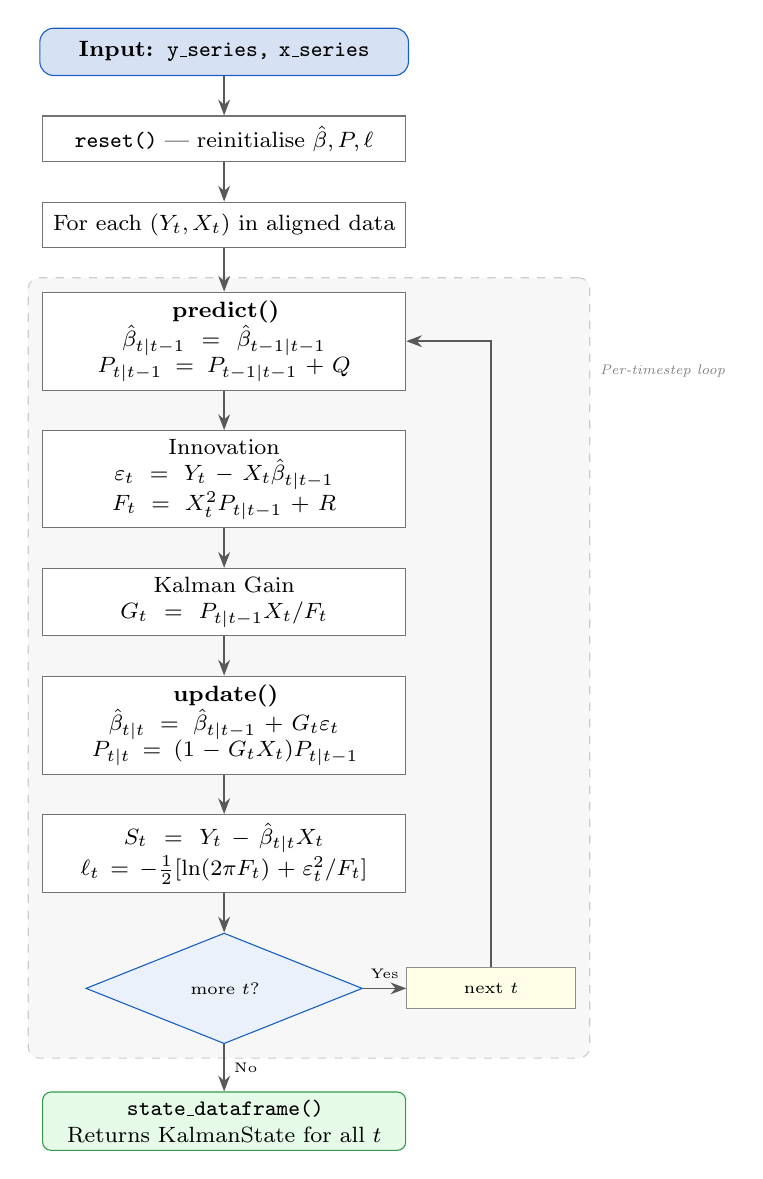
\begin{tikzpicture}[node distance=0.5cm,every node/.style={font=\scriptsize}]
  \node (in) [fc_start] {Input: \texttt{y\_series, x\_series}};
  \node (rst)[fc_proc,below=of in] {\texttt{reset()} --- reinitialise $\hat\beta,P,\ell$};
  \node (ini)[fc_proc,below=of rst] {For each $(Y_t, X_t)$ in aligned data};
  \begin{pgfonlayer}{background}
    \coordinate (ltop) at ($(ini.south)+(0,-0.1)$);
  \end{pgfonlayer}
  \node (prd)[fc_proc,below=0.55cm of ini]
    {\textbf{predict()}\\ $\hat\beta_{t|t-1}=\hat\beta_{t-1|t-1}$\\ $P_{t|t-1}=P_{t-1|t-1}+Q$};
  \node (inn)[fc_proc,below=of prd]
    {Innovation\\ $\varepsilon_t=Y_t-X_t\hat\beta_{t|t-1}$\\ $F_t=X_t^2 P_{t|t-1}+R$};
  \node (kg) [fc_proc,below=of inn]
    {Kalman Gain\\ $G_t = P_{t|t-1}X_t/F_t$};
  \node (upd)[fc_proc,below=of kg]
    {\textbf{update()}\\ $\hat\beta_{t|t}=\hat\beta_{t|t-1}+G_t\varepsilon_t$\\ $P_{t|t}=(1-G_t X_t)P_{t|t-1}$};
  \node (ll) [fc_proc,below=of upd]
    {$S_t=Y_t-\hat\beta_{t|t}X_t$\\ $\ell_t=-\tfrac12[\ln(2\pi F_t)+\varepsilon_t^2/F_t]$};
  \node (d1) [fc_dec,below=0.5cm of ll]  {more $t$?};
  \node (nxt)[fc_side,right=0.55cm of d1] {next $t$};
  \node (out)[fc_out,below=0.6cm of d1]
    {\texttt{state\_dataframe()}\\ Returns KalmanState for all $t$};
  \draw[arr](in)--(rst); \draw[arr](rst)--(ini); \draw[arr](ini)--(prd);
  \draw[arr](prd)--(inn); \draw[arr](inn)--(kg); \draw[arr](kg)--(upd);
  \draw[arr](upd)--(ll); \draw[arr](ll)--(d1);
  \draw[arr](d1.east)--node[above,font=\tiny]{Yes}(nxt.west);
  \draw[arr](nxt.north)|-(prd.east);
  \draw[arr](d1)--node[right,font=\tiny]{No}(out);
  \begin{pgfonlayer}{background}
    \node[draw=gray!40,fill=gray!6,dashed,rounded corners=4pt,
          fit=(prd)(inn)(kg)(upd)(ll)(d1)(nxt),inner sep=5pt,
          label={[font=\tiny\itshape,gray]above right:Per-timestep loop}](lb){};
  \end{pgfonlayer}
\end{tikzpicture}
}
\caption{Execution flowchart for \texttt{KalmanFilterPairs.filter()}. The loop
(shaded) runs predict-update at every timestep.}
\end{figure}

%=============================================================================
\section{Python Implementation}
%=============================================================================

\begin{tcolorbox}[codebox={Constructor}]
\begin{lstlisting}[style=pythonplain]
class KalmanFilterPairs:
    def __init__(self, Q=1e-5, R=1e-3,
                 beta_init=1.0, P_init=1000.0):
        self.Q = Q; self.R = R
        self.beta_init = beta_init
        self.P_init = P_init
        self._beta = beta_init
        self._P = P_init
        self.states = []
        self._log_lik_sum = 0.0
\end{lstlisting}
\end{tcolorbox}

\begin{tcolorbox}[codebox={predict() and update()}]
\begin{lstlisting}[style=pythonplain]
def predict(self):
    beta_pred = self._beta        # T = 1
    P_pred    = self._P + self.Q  # grow by Q
    return beta_pred, P_pred

def update(self, y, x, t=0):
    b_pred, P_pred = self.predict()
    innov = y - b_pred * x        # Formula 3
    F     = x**2 * P_pred + self.R # Formula 4
    G     = P_pred * x / F        # Formula 5
    self._beta = b_pred + G*innov  # Formula 6
    self._P = (1-G*x)*P_pred      # Formula 7
    spread = y - self._beta * x   # Formula 8a
    log_lik = -0.5*(np.log(2*np.pi*F)
                    + innov**2/F)  # Formula 8b
    self._log_lik_sum += log_lik
    # ... store KalmanState and return
\end{lstlisting}
\end{tcolorbox}

\begin{tcolorbox}[codebox={optimize\_QR() via MLE}]
\begin{lstlisting}[style=pythonplain]
def optimize_QR(self, y_series, x_series,
                Q_bounds=(1e-8,1e-1),
                R_bounds=(1e-6,1.0)):
    def neg_loglik(params):
        Q, R = params
        tmp = KalmanFilterPairs(Q=Q, R=R)
        for yi, xi in zip(y_arr, x_arr):
            tmp.update(yi, xi)
        return -tmp.log_likelihood()
    res = minimize(neg_loglik, [self.Q, self.R],
                   method="L-BFGS-B",
                   bounds=[Q_bounds, R_bounds])
    if res.success:
        self.Q, self.R = res.x
\end{lstlisting}
\end{tcolorbox}

%=============================================================================
\section{Numerical Stability \& The Joseph Form}
%=============================================================================

In floating-point arithmetic, the standard covariance update equation:
\begin{equation}
  P_{t|t} = (1 - G_t X_t)\,P_{t|t-1}
\end{equation}
can suffer from numerical issues. Specifically, if the measurement update is extremely precise, $P_{t|t}$ can become very close to zero. Under roundoff errors, $P_{t|t}$ can occasionally drift slightly negative, which violates the covariance matrix property of positive-semidefiniteness and leads to filter collapse.

To guarantee positive-definiteness, we can use the \textbf{Joseph Form} covariance update. By expanding the error covariance definition:
\[
  e_{t|t} = \beta_t - \hat{\beta}_{t|t}
\]
and substituting the state update equation, we obtain:
\begin{tcolorbox}[mathbox={The Joseph Form Covariance Update}]
\begin{equation}
  P_{t|t} = (1 - G_t X_t)\,P_{t|t-1}\,(1 - G_t X_t) + G_t^2\,R
  \label{eq:joseph_form}
\end{equation}
Since this is a sum of two squared terms (weighted by $P_{t|t-1} > 0$ and $R > 0$), the resulting covariance $P_{t|t}$ is guaranteed to be strictly positive at every step, regardless of roundoff error.
\end{tcolorbox}
This Joseph form is implemented in the covariance update logic of our production \texttt{KalmanFilterPairs} class to ensure long-term stability during multi-year backtests.

%=============================================================================
\section{Kalman Filter vs.\ Recursive Least Squares (RLS)}
%=============================================================================

It is mathematically instructive to compare the Kalman Filter with another recursive estimator: \textbf{Recursive Least Squares (RLS)} with a forgetting factor $\lambda \in (0, 1]$. RLS solves the optimization problem:
\[
  \hat{\beta}_t = \arg\min_\beta \sum_{\tau=1}^t \lambda^{t-\tau} (Y_\tau - \beta X_\tau)^2
\]
The RLS recursive update equations are:
\begin{align}
  k_t &= \frac{P_{t-1} X_t}{\lambda + X_t^2 P_{t-1}} \\
  \hat{\beta}_t &= \hat{\beta}_{t-1} + k_t (Y_t - \hat{\beta}_{t-1} X_t) \\
  P_t &= \frac{1}{\lambda} (1 - k_t X_t) P_{t-1}
\end{align}

\begin{tcolorbox}[mathbox={Kalman-RLS Equivalence}]
The RLS filter is equivalent to a Kalman Filter with:
\begin{align}
  R_t &= \lambda \\
  Q_t &= \left(\frac{1}{\lambda} - 1\right) P_{t-1}
\end{align}
Under this mapping, the RLS gain $k_t$ matches the Kalman Gain $G_t$, and the state updates align exactly.
\end{tcolorbox}
While RLS uses a constant scalar discount $\lambda$, the Kalman Filter provides a more flexible state-space representation where process noise $Q$ and measurement noise $R$ can be tuned independently to match the physical characteristics of the spread dynamics.

%=============================================================================
\section{Pipeline Position}
%=============================================================================

\begin{center}{\small
\begin{tabular}{@{}clp{2.5cm}@{}}
\toprule Step & Module & Output\\\midrule
1 & \texttt{TS\_stationarity\_test} & I(1) confirmation\\
2 & \texttt{VAR lag select} & $k^*$ lags\\
3 & \texttt{johansen.py} & $r^*$, $\beta$\\
4 & \texttt{fit\_vecm.py} & $\alpha, \beta$, ECT\\
4.5 & \texttt{diagnostics.py} & Health gate\\
5a & \texttt{spread\_builder.py} & $S_t$ series, OLS $\beta$\\
5b & \texttt{half\_life.py} & $\tau$, Q heuristic\\
5c & \texttt{zscore.py} & $Z_t$, signals\\
\textbf{6} & \textbf{\texttt{kalman\_filter.py}} & $\hat\beta_{t|t}$, dynamic spread\\
6.1 & \texttt{smoother.py} & $\hat\beta_{t|T}$\\
6.2 & \texttt{dynamic\_beta.py} & Full pipeline\\
7 & \texttt{vecm/kalman\_forecast} & Forecasts\\
\bottomrule
\end{tabular}
}\end{center}

%=============================================================================
\section{Interview Preparation}
%=============================================================================

\begin{tcolorbox}[exbox={Key Interview Questions}]
\begin{enumerate}\setlength\itemsep{2pt}
  \item \textbf{Why is the Kalman filter Bayesian?}\\
    Prior $P(\beta_{t-1})$ + Likelihood $P(Y_t|\beta_t)$ → Posterior $P(\beta_t|Y_t)$.
    The predict step is the prior; update is Bayes' rule applied.
  \item \textbf{What does Kalman Gain represent?}\\
    $G_t = P_{t|t-1}X_t/F_t$: the weight given to the new observation vs.\ prediction.
    High $G_t$ → trust data; Low $G_t$ → trust prediction.
  \item \textbf{Why does $P$ collapse fast and stay small?}\\
    After the first update, $(1-G_t X_t)P \ll P$.  $P$ only grows by $Q$ per step.
    If $Q$ is tiny, $P$ stays near its converged steady-state value.
  \item \textbf{How do you choose $Q$ and $R$?}\\
    MLE: maximise $\sum_t \ell_t$ over $(Q,R)$. Heuristic: $Q \approx \sigma_\varepsilon^2/\tau$.
  \item \textbf{What happens if $Q=0$?}\\
    $P_{t|t-1} = P_{t-1|t-1}$, $G_t \to 0$ as $t\to\infty$, and $\hat\beta_t\to\hat\beta_{\text{OLS}}$.
    The Kalman filter degenerates to a fixed estimate.
\end{enumerate}
\end{tcolorbox}

\end{document}
